\title{Recurrent Neural Network Emulation of Turbulent Geophysical Fluids}

\author{Timothy A. Smith$^{1,2}$, \texttt{tim.smith@noaa.gov}\vspace{-.25em}}

\begin{minipage}{.5\textwidth}
    \vspace{-1.75em}
    \author{Stephen G. Penny$^{3}$\vspace{.25em}}
    \author{Jason A. Platt$^{4}$\vspace{.25em}}
    \author{Tse-Chun Chen$^{1,2}$}
\end{minipage}
\begin{minipage}{.5\textwidth}
    \institution{\fontsizeinstitution
        \justifying
        $^1$CIRES, CU Boulder \\
        $^2$NOAA, Physical Sciences Lab (PSL) \\
        $^3$Sofar Ocean Technologies\\
        $^4$University of California, San Diego
    }
\end{minipage}

\section{Motivating Goals}
\begin{itemize}
    \item Develop cheap emulator to replace General\\Circulation Models (GCMs) in Data Assimilation (DA)
    \item Enable increased ensemble size and/or resolution
\end{itemize}

\section{Why use RNNs?}
\begin{itemize}
    \item Recurrent Neural Networks (RNNs) discussed here have achieved excellent
        prediction skill emulating chaotic dynamics \cite{platt_systematic_2022}
    \item For low dimensional chaotic systems, successful
\end{itemize}

\hfill\begin{minipage}{.95\textwidth}
    \begin{enumerate}
        \item Lyapunov spectrum reproduction\cite{pathak_using_2017}
        \item Numerical model replacement in DA algorithms
            \cite{penny_integrating_2022}
    \end{enumerate}
\end{minipage}

\section{Questions to be Addressed}
\begin{itemize}
    \item What scales can we truly resolve with neural\\network emulators?
    \item How do fundamental data decisions impact\\performance?
    \item How does memory, a unique but costly RNN feature, benefit performance?
\end{itemize}

\section{Surface Quasi-Geostrophic Turbulence}

\vspace{1em}
\begin{minipage}{.6\textwidth}
    \begin{tikzpicture}[scale=1]
        \node(upper) at (-1, 1){
            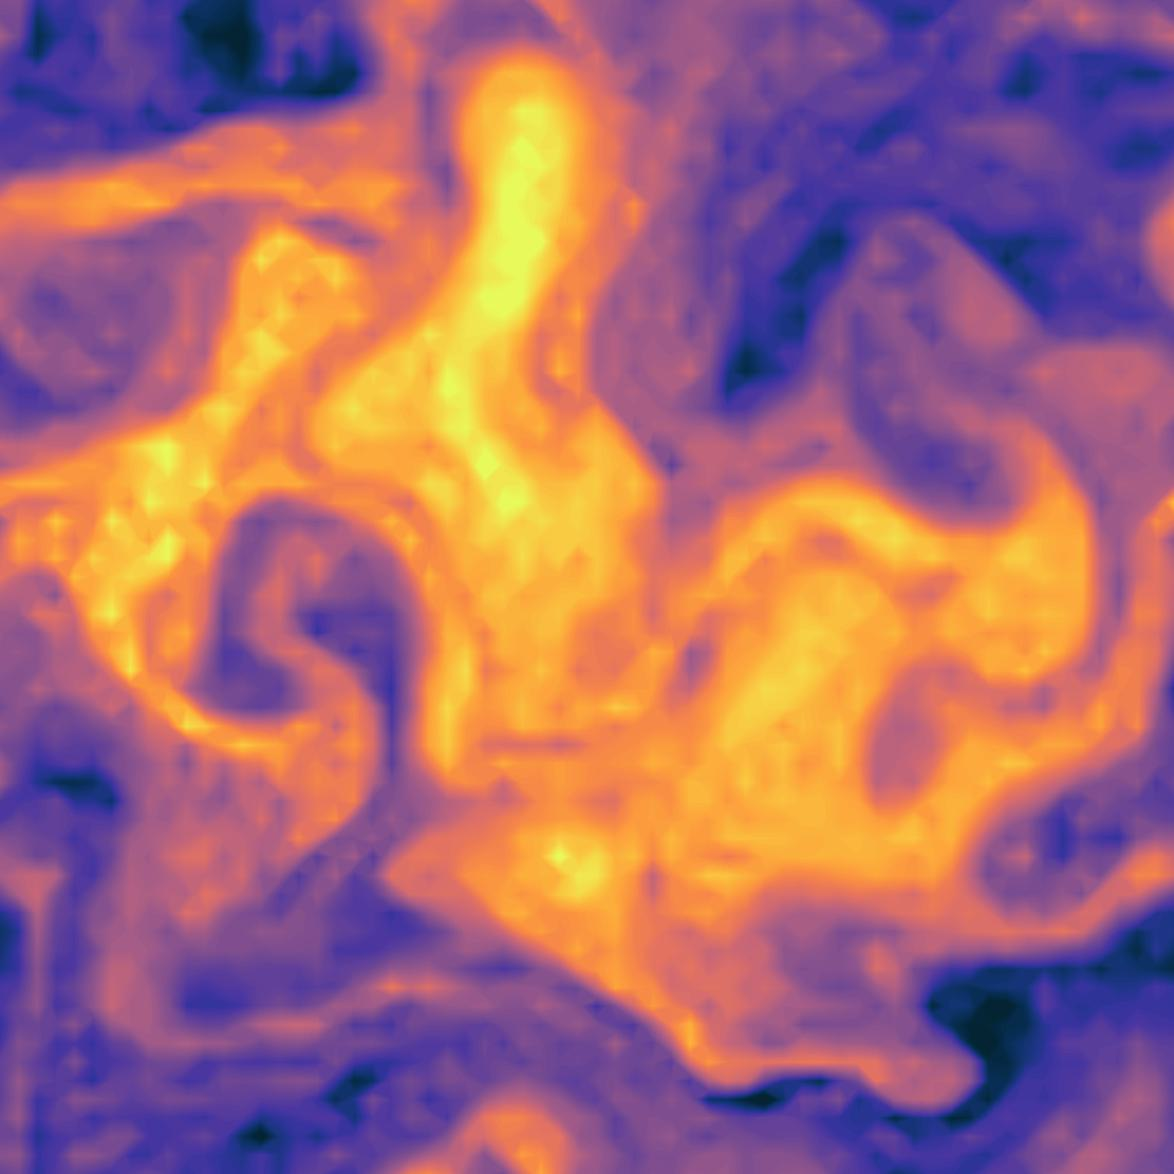
\includegraphics[width=.74\textwidth]{../../figures/theta-z1.jpg}
        };
        \node(lower) at (1, -1){
            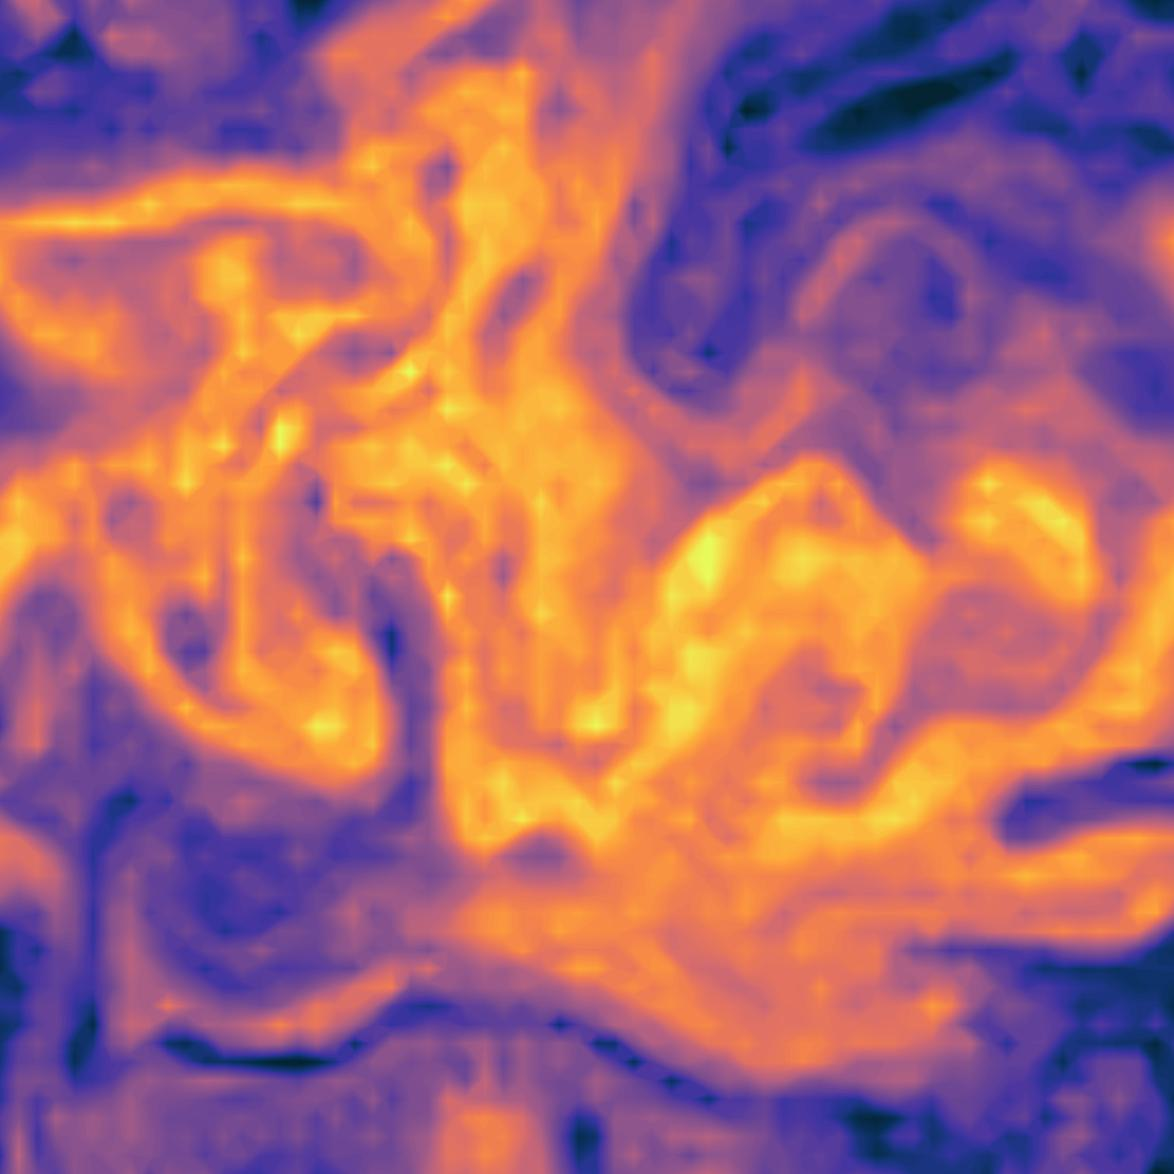
\includegraphics[width=.74\textwidth]{../../figures/theta-z0.jpg}
        };
        \draw [line width=5pt,
            {Stealth}-{Stealth}]
            ($ (lower.south west) + (0.45, 0.0) $)
            --
            ($ (lower.south east) - (0.45, 0.0) $)
            node [midway, yshift=-0.75em] {$N_x = 64$};
        \draw [line width=5pt,
            {Stealth}-{Stealth}]
            ($ (upper.south west) + (0.0, 0.45) $)
            --
            ($ (upper.north west) - (0.0, 0.45) $)
            node [midway, xshift=-0.75em, rotate=90] {$N_y = 64$};
        \draw [line width=5pt,
            {Stealth}-{Stealth}]
            (upper.south west)
            --
            (lower.south west)
            node [midway, xshift=-0.5em, yshift=-0.5em, rotate=-45] {$N_z = 2$};
    \end{tikzpicture}
\end{minipage}
\begin{minipage}{.39\textwidth}
    \begin{itemize}
        \item Blumen model of Eady turbulence, as presented in\\
            \cite{tulloch_note_2009}
        \item 15 years: training and validation
        \item 5 years: testing
        \item 5 years: separation
    \end{itemize}
\end{minipage}
